% Model. Sources: refs/docs/model_arch.md §1--5, refs/docs/task_prompts.md; HTML §3.
% Structure follows the encoder + LLM overview with a module table (1.0 report §4,
% Qwen3-ASR technical report), per AGENTS.md rule 6.

\section{Model}
\label{sec:model}

\subsection{Overview}
\label{subsec:model_overview}

AmphionASR~2.0 consists of an audio encoder and a language model, both initialized from Qwen3-ASR-1.7B~\cite{shi2026qwen3asr}.
The audio encoder, AuT, consists of convolutional downsampling and a 24-layer Transformer; it maps the 128-dimensional Mel features of 16\,kHz mono audio to 12.5\,Hz frame embeddings, which are projected into the language model.
Following SpeechLLM convention, we call it a 1.7\,B model after the size of its language model; \Cref{tab:params} lists the parameter counts.

\begin{table}[t]
  \caption{Parameter counts of AmphionASR~2.0.}
  \label{tab:params}
  \centering
  \small
  \begin{tabularx}{\linewidth}{@{}llX@{}}
    \toprule
    Component & Parameters & Notes \\
    \midrule
    Audio encoder (AuT) & about 300\,M & Initialized from the AuT encoder of Qwen3-ASR-1.7B: convolutional downsampling and a 24-layer Transformer, 1024-dimensional, 12.5\,Hz \\
    Separator vector \septok & 1{,}024 & Inserted between the enrollment and mixture segments after the convolution and before the Transformer, in TS-ASR mode only; trainable \\
    Language model & 1.7\,B & Initialized from the language model of Qwen3-ASR-1.7B: 28-layer decoder, 2048-dimensional \\
    \midrule
    Total & about 2.0\,B & Called a 1.7\,B model by convention, after the size of its language model \\
    \bottomrule
  \end{tabularx}
\end{table}

\subsection{Target-speaker input construction}
\label{subsec:model_input}

\Cref{fig:input} shows how the enrollment and the mixture enter the model in TS-ASR mode.

\begin{figure}[t]
  \centering
  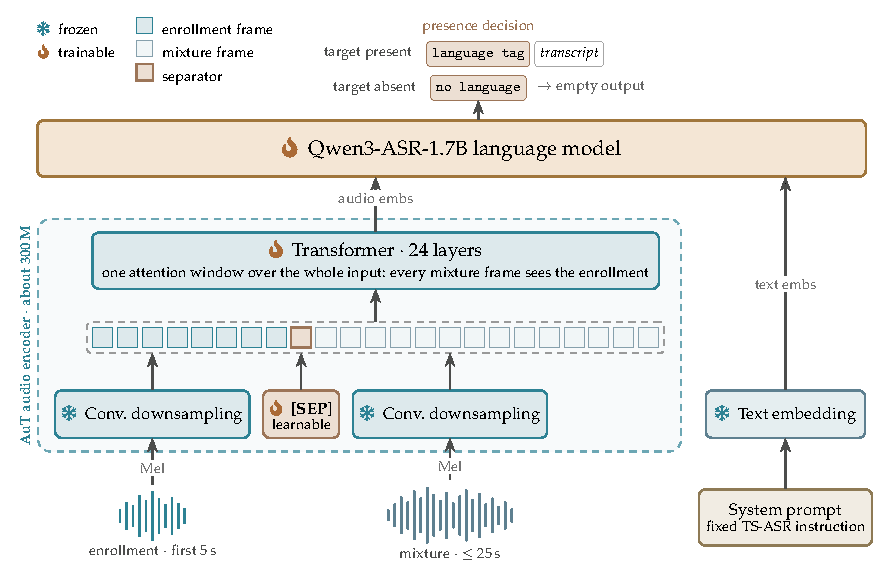
\includegraphics[width=\linewidth]{figures/input-construction.pdf}
  \caption{AmphionASR~2.0 in TS-ASR mode. The enrollment (first 5\,s) and the mixture (at most 25\,s) get separate Mel features and pass separately through the frozen convolutional downsampling of the AuT encoder. After the convolution, a learnable \septok vector joins them into one sequence before the 24 Transformer layers, whose attention covers the whole input. The fixed system prompt enters the language model through the frozen text embedding, and the language tag at the start of the output carries the present or absent decision.}
  \label{fig:input}
\end{figure}

\paragraph{Separate convolution.}
Each segment gets its own Mel features, is zero-padded to a whole number of Mel hops and passes through the convolutional downsampling of AuT on its own, with its own positional encoding.
The last enrollment frame and the first mixture frame therefore never share a convolutional receptive field.
The convolution layers stay frozen during fine-tuning.

\paragraph{A learnable separator.}
\septok is a trainable 1024-dimensional vector and is inserted only in TS-ASR mode; plain and hotword ASR neither split the input nor insert it.
The language model thus receives one audio token for each convolutional output of the enrollment and the mixture, plus one for \septok.

\paragraph{Global attention.}
The Qwen3-ASR encoder supports chunked attention windows of 1--8\,s~\cite{shi2026qwen3asr}.
With chunking, mixture frames far from the enrollment could not attend to it, so both training and inference use a single window that covers the whole input.
Every mixture frame can attend to the enrollment segment in every layer.

\paragraph{Empty output.}
When the target is present, the model outputs a language tag followed by the transcript; when the target is absent, the tag marks no language and the transcript is empty.
The presence decision is concentrated on this tag, so an application can set a more conservative threshold on its probability.

\subsection{Task formats}
\label{subsec:model_tasks}

The three tasks share all parameters and differ only in the system prompt and in the audio layout (\Cref{tab:tasks}).
A 5\,s enrollment is recommended, and 3\,s is also supported.
One request carries at most 30\,s of audio, so in TS-ASR mode the mixture is at most 30\,s minus the enrollment length; longer recordings must be segmented first.

\begin{table}[t]
  \caption{Input format of the three tasks.}
  \label{tab:tasks}
  \centering
  \small
  \begin{tabularx}{\linewidth}{@{}l>{\raggedright\arraybackslash}Xl@{}}
    \toprule
    Task & System prompt & Audio \\
    \midrule
    Plain ASR & empty & whole clip, $\le$ 30\,s \\
    Hotword ASR & list of hotwords & whole clip, $\le$ 30\,s \\
    TS-ASR & fixed instruction & enrollment (first 5\,s) + \septok + mixture ($\le$ 25\,s) \\
    \bottomrule
  \end{tabularx}
\end{table}
